\begin{figure*}[htb]
  \vspace{-0.6cm}
  \centering
  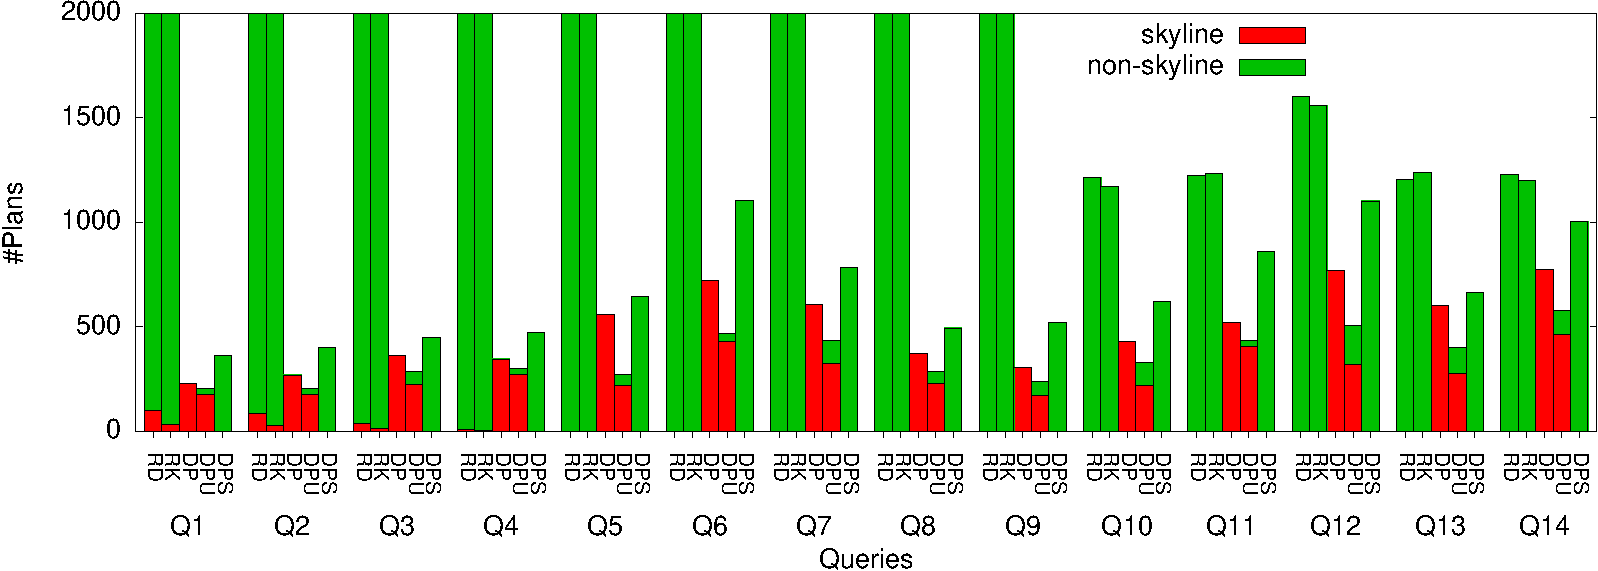
\includegraphics[width=0.75\linewidth]{figs/all_queries-crop.pdf}
  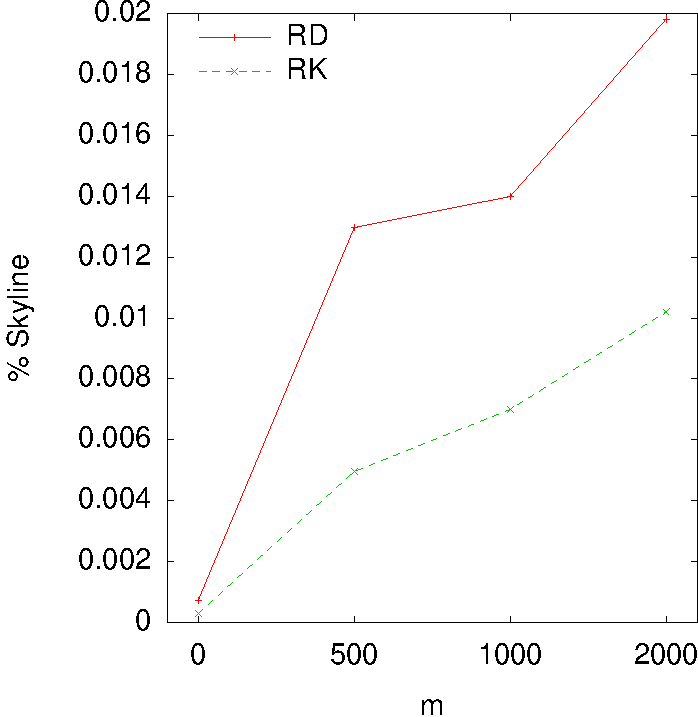
\includegraphics[width=0.24\linewidth]{figs/plans_skyline_by_m-crop.pdf}
  \caption{a) Number of skyline and non-skyline plans for all queries
    and systems ($b=0.8, m=2000$), b) Skyline fraction for RD, RK for
    different value of $m$ ($b=0.8$).}
  \label{fig:queries}
  \vspace{-0.5cm}
\end{figure*}

\section{Evaluation}
\label{sec:eva}
Existing works in data integration~\cite{levy_querying_1996} and Linked Data query processing~\cite{harth_data_2010,ladwig_linked_2010} perform source ranking
without further optimization. We implement source ranking to select sources first, and then use the dynamic DP solution as proposed for Linked Data query optimization to optimize
the subsequent process. That is, the proposed query plan as well as
the operator sharing mechanism are employed to optimize cost. This is
to obtain a best-effort baseline, based on which we aim the study of
effect of the holistic treatment of source selection and query
processing, and the multi-objective optimization we propose. The
experiment shows that as opposed to our approach, the baseline yields
only a small fraction of the complete set of Pareto-optimal plans, and
the resulting suboptimal plans lead to much higher total cost when producing
the same number of results. 

%Compared to the baseline, resulting cost (measured in terms of total time needed for computing results) needed may be as 

%The evaluation of our approach consists of two parts. In the first, we
%evalute the benefit of using the dynamic programming query
%optimization algorithm for Linked Data query processing in a
%single-objective scenario. In the second part, we focus on the
%multi-objective optimization approach proposed in this paper.

% \subsection{Single-objective Optimization with Dynamic Programming}

% \subsubsection{Systems}


% \subsubsection{Results}



% \begin{figure}[htb]
%   \centering
%   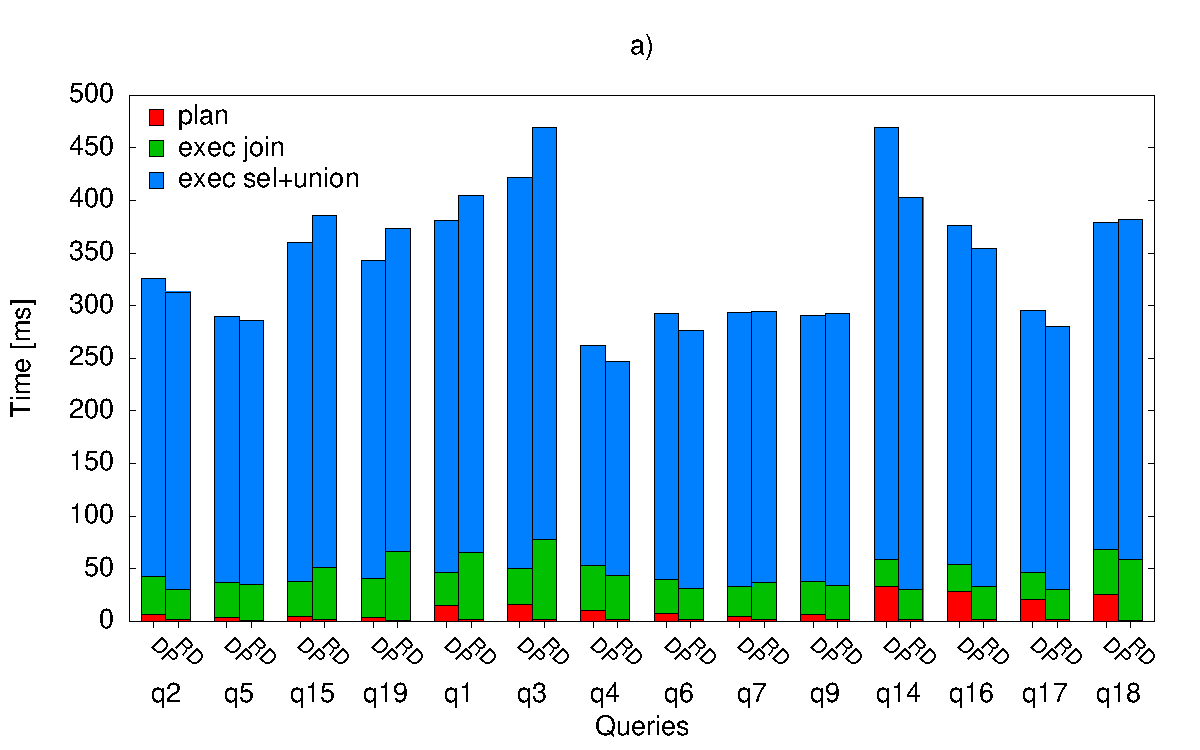
\includegraphics[width=\linewidth]{figs/exec_queries.pdf}
%   \caption{Results for execution}
%   \label{fig:exec_queries}
% \end{figure}



\subsection{Systems}
\textbf{Our Approach.} We implemented three versions of our
approach. The first version (DP) implements all the proposed
techniques to produce the complete set of Pareto-optimal plans. The
second version (DPU) also uses operator sharing such that for
subsequent source accesses, the refined cost model applies. However,
the effect of this is not taken into account during pruning.  That is,
it uses directly the cost instead of the lower and upper bounds that
have been established to guarantee monotonicity of cost. Thus, at the
cost of compromising Pareto-optimality, DPU can prune more
aggressively and thus, is expected to exhibit better performance. This baseline can be seen as an approximate version of our approach that simply uses actual cost as an approximate estimate for bounds. 
%With
%this baseline, we aim to study the positive effect of using the
%proposed bounds on Pareto-optimality, and to find out whether the
%proposed technique for estimating the bounds is effective in reducing
%the overhead resulting from that. 
The third version (DPS) does not use
operator sharing at all, i.e. if a source is used for more than one
triple pattern it is retrieved multiple times. 
%We use DPS to study the effect the benefits operator sharing.
We use different settings for $b$ to study the effect of operator sharing. For example, with $b=0.8$ the optimizer assumes that 80\% of
the source scan cost is saved, i.e. subsequent reads cost only 20\% of the first read.

\textbf{Baselines.} Existing Linked Data approaches implement ad-hoc
source ranking to select few best
sources~\cite{harth_data_2010,ladwig_linked_2010}, and then process
these sources without further optimization. This processing represents
one single plan, whose optimality is unknown. We implement this source
ranking (RK) and a random source selection strategy (RD), and 
%Given the
%selected sources, 
apply our DP solution on top but only to
optimize the cost. 
% these baselines need to produce results from these
%sources. 
%In the same way proposed for our approach, this DP solution
%applies operator sharing so that sources can be reused. 
Instead of one
single cost-optimized plan, our approach however yields a Pareto-set
of query plans that represents different trade-offs between cost and
cardinality. Thus, we further extend these baselines to use different
combinations of sources that yield different plans.

Both baselines first retrieve all relevant sources $D$ for a query $Q$
from the source index, i.e. $D = \bigcup_{t \in Q} source(t)$. Then,
a set $\mathcal{D}$ containing $|D|$ different subsets of $D$, each
with size in the range $[1,|D|]$ is created.
%The number of  captured by and $|\mathcal{D}| = |D|$. 
The baselines differ in how these
subsets are selected:
\begin{itemize}
\item Baseline RD randomly selects the $|D|$ subsets.
\item Baseline RK first ranks sources in $D$ by the number of
  contained triples that match query triple patterns, calculated as
  $score(d) = \sum_{t \in q} card_d(t)$. The subsets are created by
  starting with the highest ranked source and then successively adding
  sources in the order of their rank to obtain $|D|$ subsets in total.
\end{itemize}
Each element in $\mathcal{D}$ represents a combination of sources, for
each of which a query plan is created. As a result, we have a set of
plans, which vary in the number of results as well as cost because
different combinations of sources are used.
% using a standard dynamic
%programming optimizer (i.e., no multi-objective optimization). Sharing
%of source scan operators is also employed where possible.

Note that our approach not only selects sources (source scan
operators) but also for which triple patterns these sources are used
(selection operators), while the sources selected for the baselines
are used for all triple patterns. In order to obtain even more plans
that further vary in the number of results they produce, we create an
additional set of $m$ plans for each previously created plan of the
baselines RK and RD by
randomly removing a subset of the inputs (selection operators) from
the unions at the root of their access plans.
%In particular, to create a new plan from an
%existing plan, for each union that is root of an access plan, we
%remove a random subset of its input (selection) operators. 
%If the source scan operator that is input for a removed selection operator is
%not shared it is also remove from the plan.
%Any invalid plans that are constructed in this way (e.g., all inputs of an union might have been) are discarded. 
In the end, each baseline has at most $m \cdot |D|$ plans that vary
in terms of results (of which only $|D|$ plans actually vary in cost).

%These baselines optimize source selection independent from the
%subsequent computation of results. While the goal of source selection
%is to choose those that contribute many results, the subsequent
%optimization focuses on cost. Compared to them, our approach not only
%jointly optimize sources section and result computation but also,
%considers cardinality and cost at the same time. Our goal is to study
%the effect of this joint optimization on the Pareto-optimality of
%plans. Further, we will investigate the effect of using non-optimal
%plans on the result....
%While this effect is expected to be positive, the increased complexity of the planning problem also leads to additional cost. Thus, we will also investigate whether this overhead can be justified by looking at the total processing time needed for producing several fixed fraction of results.  

%
%\textbf{Parameters.} Parameter $b$ specifies the benefit that is
%assumed during query planning for sharing of source scan
%operators. For example, with $b=0.8$ the planners assume that 80\% of
%the source scan cost is saved, i.e., second and subsequent reads of a
%source scan operator cost only 20\% of the first read.
%
%For RD and RK, parameter $m$ describes the number of additional plans
%that were generated by randomly remove selection and source scan
%operators.

\begin{figure}[htb]
  \vspace{-0.1cm}
  \centering
  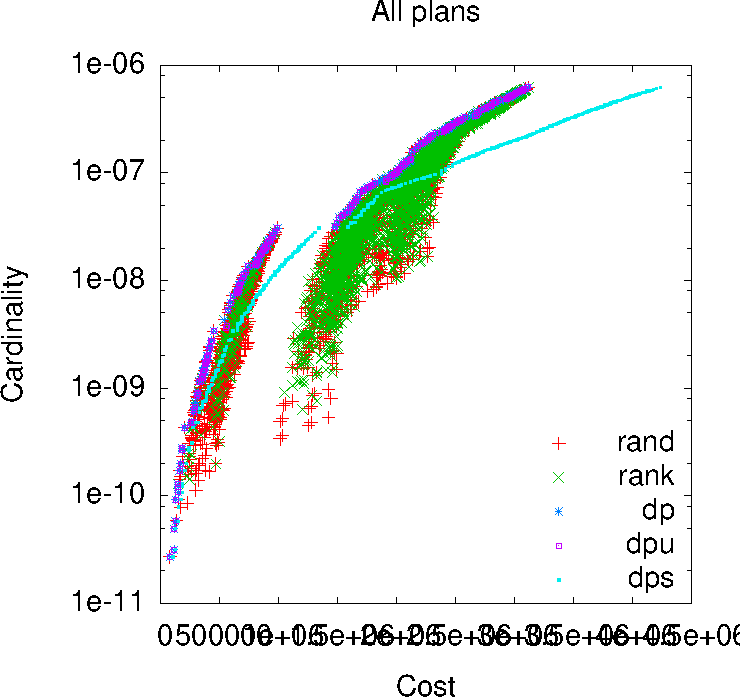
\includegraphics[width=0.48\linewidth]{figs/plans_q2_all-crop.pdf}
  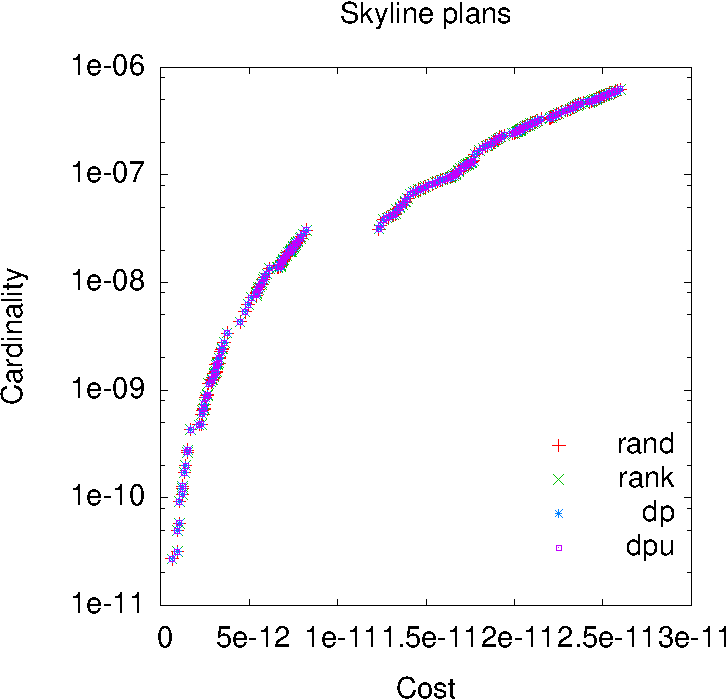
\includegraphics[width=0.48\linewidth]{figs/plans_q2_sky-crop.pdf}
  \caption{Plans for query Q1 on all systems: a) all plans and b)
    skyline plans ($b=0.8,m=2000$).}
  \label{fig:pareto_q2_skyline}
  \vspace{-0.5cm}
\end{figure}

\subsection{Setting} As data, we use real-world Linked Data currently available on the Web. We generate queries and process them against Linked Data sources on the Web to obtain a total of 1,909,109 triples from various popular datasets such as DBpedia, Freebase, New York Times, GeoNames and LinkedMDB. The number of Linked Data sources from which all data were retrieved is 516,293. During this process, we observed that network latency greatly varies. In order to systematically study the effects of query processing, we thus decided to download these data, and to simulate Linked Data query processing on one single machine. To reflect network cost, we tried different settings, including the average of 1.5s that we could observed on real-world sources. Performance differences between systems were however not sensitive to these settings. 

As queries, we focus on 14 BGP queries that have non-empty results. The result size is in the range from 1 to 836. We use queries that largely differ in the number of results to discuss the effect of Pareto-optimality on the cost-cardinality trade-off in detail. These queries belong to different classes of complexity, which is reflected in the number of triple patterns. For the classes of 3, 4 and 5 patterns, we have 4, 5, and 5 queries, respectively. 


%Table~\ref{tab:queries} shows various
%statistics for all evaluation queries.

%This dataset was then
%indexed in a source index and used for the evaluation. 
%As the source index contained too many sources for the multi-objective
%optimization approach to deal with, we randomly aggregated sources
%during the creation of access plans into a set of $k=5$ virtual
%sources. The size of the virtual sources follows a Zipf distribution
%with exponent $2$.


%
%\begin{table}[htb]
%  \centering
%  \begin{tabular}{l|c|c|r}
%    Query & \#Pat. & Shared [kT] & \#Res. \\%& Join-Sel. SD \\ 
%    \hline
%
%    Q2  & 3 & 1,393 & 24  \\%& 3.26\textsc{e}-5 \\
%    Q5  & 3 & 1,425 & 13  \\%& 4.95\textsc{e}-5 \\
%    Q15 & 3 & 1,401 & 11  \\%& 2.59\textsc{e}-5 \\
%    Q19 & 3 & 1,434 & 836 \\%& 4.36\textsc{e}-5 \\
%    \hline
%    Q1  & 4 & 1,426 & 2   \\%& 1.30\textsc{e}-3 \\
%    Q3  & 4 & 1,892 & 3   \\%& 1.89\textsc{e}-5 \\
%    Q4  & 4 & 1,415 & 60  \\%& 9.58\textsc{e}-3 \\
%    Q6  & 4 & 2,081 & 6   \\%& 2.62\textsc{e}-3 \\
%    Q7  & 4 & 1,369 & 106 \\%& 2.75\textsc{e}-3 \\
%    \hline
%    Q9  & 5 & 1,405 & 17  \\%& 5.26\textsc{e}-3 \\
%    Q14 & 5 & 1,830 & 20  \\%& 3.71\textsc{e}-3 \\
%    Q16 & 5 & 2,396 & 1   \\%& 2.10\textsc{e}-3 \\
%    Q17 & 5 & 1,409 & 1   \\%& 8.92\textsc{e}-3 \\
%    Q18 & 5 & 1,007 & 2   \\%& 1.21\textsc{e}-4 \\
%  \end{tabular}
%  \caption{Query statistics: query name, number of patterns, number of
%    triples (in thousands) contained in shared sources, number of results.}
%  \label{tab:queries}
%\end{table}

% \begin{table*}[htb]
%   \centering
%   \begin{tabular}{l|r|r|r|r|r|r|r|r|r|r|r|r|r|r|r|r}
%  & RD & RK & DP & DPU & RD & RK & DP & DPU & RD & RK & DP & DPU & RD & RK & DP & DPU \\
%     \hline               
                                                                                                               
%  & \multicolumn{4}{c}{Q2} & \multicolumn{4}{|c|}{Q5} & \multicolumn{4}{c}{Q15} & \multicolumn{4}{|c}{Q19}  \\

%     \hline                                                                                                   

%     \#Plans   & 1702 & 1853 & 673   & 619  & 1382 & 1871 & 446   & 446   & 2376 & 3263 & 634   & 634   & 3817 & 3240 & 761   & 761   \\
%     \#Skyline & 153  & 155  & 673   & 575  & 106  & 176  & 446   & 446   & 13   & 40   & 634   & 634   & 41   & 46   & 761   & 761   \\ 
%     \%Skyline & 22.7 & 23.0 & 100.0 & 85.4 & 23.8 & 39.5 & 100.0 & 100.0 & 2.1  & 6.3  & 100.0 & 100.0 & 5.4  & 6.0  & 100.0 & 100.0 \\
%     Time [s]  & 1.06 & 0.92 & 1.14  & 0.62 & 0.78 & 1.03 & 0.75  & 0.53  & 1.05 & 1.14 & 1.21  & 0.64  & 1.07 & 1.05 & 1.58  & 0.77  \\
  
%     \hline
%     \hline

%  & \multicolumn{4}{c}{Q1} & \multicolumn{4}{|c|}{Q3} & \multicolumn{4}{c|}{Q4} & \multicolumn{4}{c}{Q6} \\

%     \hline

%     \#Plans   & 3945 & 5362 & 866   & 832  & 4571 & 5153 & 901   & 847  & 1471 & 1306 & 453   & 465  & 954  & 1340 & 354   & 318  \\
%     \#Skyline & 0    & 0    & 866   & 689  & 0    & 0    & 901   & 699  & 1    & 0    & 453   & 434  & 0    & 1    & 354   & 283  \\ 
%     \%Skyline & 0.0  & 0.0  & 100.0 & 79.6 & 0.0  & 0.0  & 100.0 & 77.6 & 0.2  & 0.0  & 100.0 & 95.8 & 0.0  & 0.2  & 100.0 & 79.9 \\
%     Time [s]  & 1.53 & 1.67 & 7.64  & 1.60 & 1.53 & 1.62 & 10.05 & 1.80 & 1.61 & 1.29 & 1.37  & 0.75 & 1.14 & 1.33 & 1.35  & 0.70 \\

%     \hline
%     \hline

%  & \multicolumn{4}{c}{Q7} & \multicolumn{4}{|c|}{Q9} & \multicolumn{4}{c|}{Q14} & \multicolumn{4}{c}{Q16} \\

%     \hline

%     \#Plans   & 2566 & 3913 & 1035  & 813  & 2622 & 3450 & 689   & 655  & 429  & 436  & 284   & 281  & 1485 & 2265 & 685   & 663  \\
%     \#Skyline & 1    & 0    & 1035  & 781  & 0    & 0    & 689   & 637  & 0    & 0    & 284   & 281  & 0    & 0    & 685   & 583  \\ 
%     \%Skyline & 0.1  & 0.0  & 100.0 & 75.5 & 0.0  & 0.0  & 100.0 & 92.5 & 0.0  & 0.0  & 100.0 & 98.9 & 0.0  & 0.0  & 100.0 & 85.1 \\
%     Time [s]  & 1.91 & 1.50 & 20.88 & 2.28 & 1.80 & 1.64 & 23.64 & 2.56 & 1.33 & 1.21 & 0.91  & 0.41 & 1.82 & 1.99 & 14.31 & 2.38 \\

%     \hline
%     \hline

%  & \multicolumn{4}{c}{Q17} & \multicolumn{4}{|c|}{Q18} & \multicolumn{8}{c}{} \\

%     \hline

%     \#Plans   & 837  & 1022 & 398   & 286   & 1021 & 1192 & 633   & 633   & \multicolumn{8}{c}{} \\
%     \#Skyline & 1    & 0    & 398   & 286   & 0    & 0    & 633   & 633   & \multicolumn{8}{c}{} \\ 
%     \%Skyline & 0.2  & 0.0  & 100.0 & 100.0 & 0.0  & 0.0  & 100.0 & 100.0 & \multicolumn{8}{c}{} \\
%     Time [ms] & 1.67 & 1.70 & 2.68  & 0.66  & 1.53 & 1.58 & 4.15  & 1.35  & \multicolumn{8}{c}{} \\

%   \end{tabular}
%   \caption{Results for all queries, with $m=2000$ and $b=0.8$ for RD and RK.}
%   \label{tab:res}
% \end{table*}

%\subsection{Setting}
All systems were implemented in Java.  All experiments were executed
on a 2009 Macbook Pro with a 2.4 GHz Intel Core 2 Duo processor, 4GB
RAM (of which 1GB was assigned to the Java VM) and a Crucial m4 128GB
SSD.
\begin{figure*}[htb]
  \vspace{-0.6cm}
  \centering
  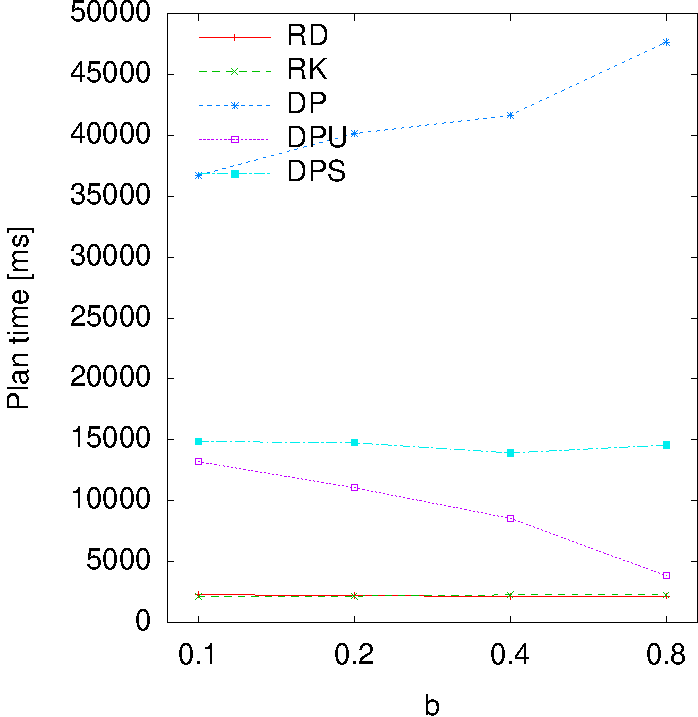
\includegraphics[width=0.24\linewidth]{figs/pareto_plan_b-crop.pdf}
  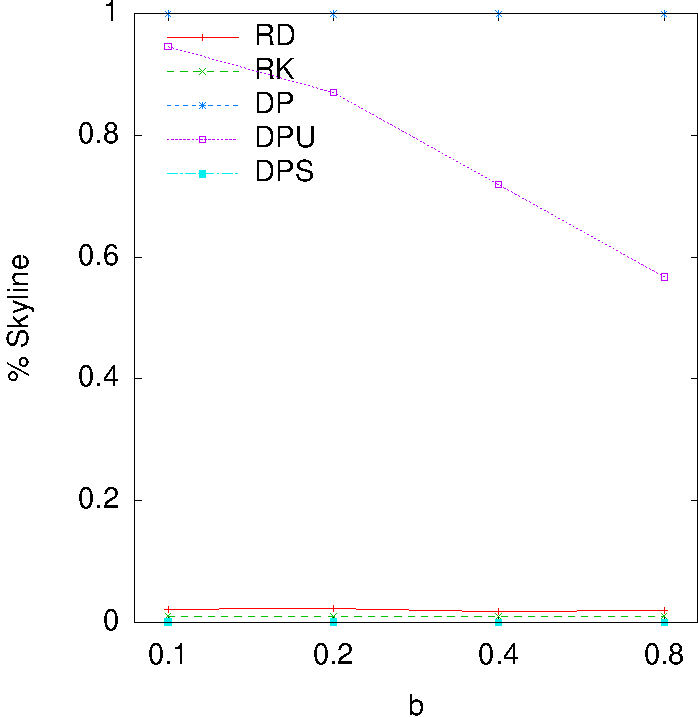
\includegraphics[width=0.24\linewidth]{figs/plans_skyline_by_b-crop.pdf}
  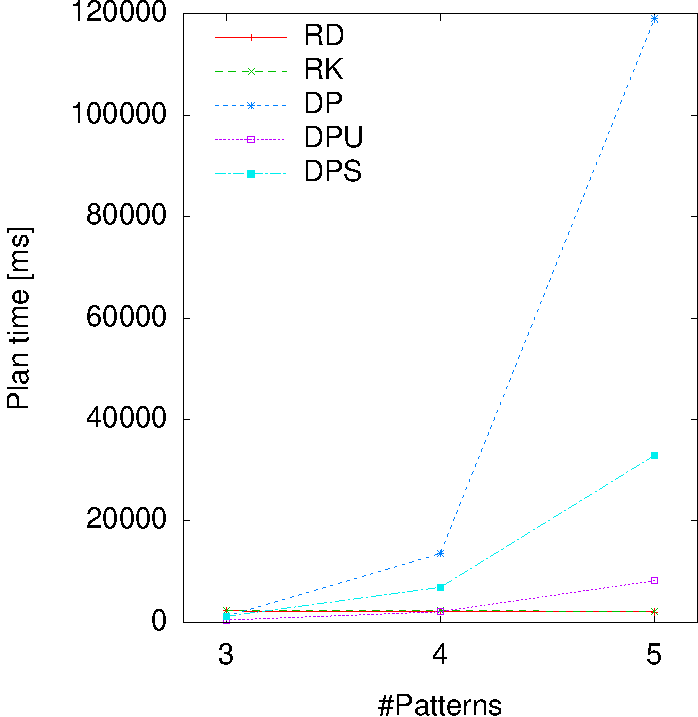
\includegraphics[width=0.24\linewidth]{figs/pareto_plan_tp-crop.pdf}
  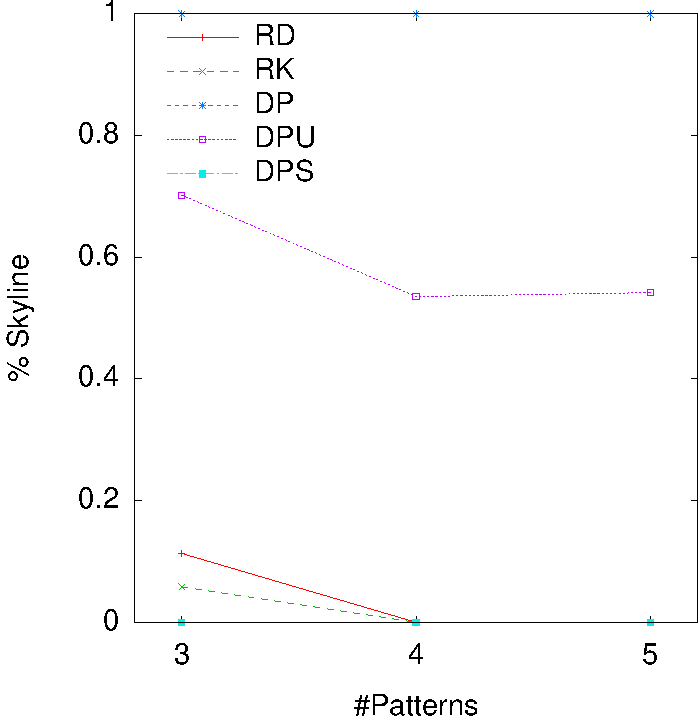
\includegraphics[width=0.24\linewidth]{figs/plans_skyline_by_tp-crop.pdf}
  \caption{Effect of sharing benefit on a) planning time and b)
    skyline fractions ($m=2000$). Effect of query complexity on c) planning time and d) skyline
     fractions ($b=0.8, m=2000$).}
  \label{fig:pareto_sharing}
  \vspace{-0.5cm}
\end{figure*}


\subsection{Results}
Fig.~\ref{fig:queries}a shows an overview of all queries and displays
the number of plans that were generated by each system, categorized
into skyline and non-skyline (i.e.  dominated) plans. The skyline
plans were determined by collecting all plans of a particular query
for all systems and then pruning all dominated plans.

We can see that DP produces only skyline plans and that there are many
DPU plans that are part of the skyline (56\% on average). However, the
RD and RK baselines generate only small fractions of skyline plans
(1.9\% and 1\% on average). DPS finds only few skyline plans (less the
1\%).

Fig.~\ref{fig:queries}b shows the skyline fraction for RD and RK for
values of $m$. For larger values the skyline fraction is
higher, meaning that the larger plan space created by randomly
removing union inputs is necessary to find skyline plans.

Figs.~\ref{fig:pareto_q2_skyline}a+b show a scatter plot of cost and
cardinality of plans generated by all systems for query Q1. In these
plots a plan dominates all other plans that are to its lower right,
i.e. that have higher cost (x-axis) and lower cardinality
(y-axis). Fig.~\ref{fig:pareto_q2_skyline}a shows all plans that were
generated by the different systems. We can immediately see that many
of the plans generated by the RD and RK baselines are dominated by
other plans and that all DPS plans are also
suboptimal. Fig.~\ref{fig:pareto_q2_skyline}b shows for all systems
only the plans that are on the skyline. Here, the dominated DPS plans
no longer appear and only few RD and RK plans remain.


Note that RD simply reflects the number of plans that are randomly
generated. Out of the 3,154 random plans generated on average, only
1\% are optimal. This suggests that the total space of plans is large,
and a correspondingly large amount of plans have to be generated for
RD to have higher coverage of optimal plans. Ranking sources based on
cardinality only does not help to produce Pareto-optimal plans. In
fact, we can see that this bias towards cardinality as reflected by
the RK baseline actually leads to a smaller amount of optimal plans,
compared to the random strategy (Fig.~\ref{fig:queries}b). DPU
optimizes for both objectives, thus is able to produce better
trade-offs than RK and RD in most cases
(Fig.~\ref{fig:pareto_q2_skyline}a). However, because it
systematically uses the wrong estimate for cost, the resulting plans
are relatively ``good'' but rarely optimal.


\textbf{Effect of Query Complexity.} Figs.~\ref{fig:pareto_sharing}c+d show 
planning time and skyline fraction for different number of triple patterns. An increased number of triple
patterns results in a larger search space for the query optimizer. This intuition is supported by the results, which show that both performance and quality decrease with increasing number of patterns. 

Whereas for 3 triple patterns the baselines RD and RK are able to find 11\% and 6\% of the skyline plans, few
are found for 4 and 5 triple patterns (< 1\%). DPU provides 
70\% of the skyline for 3 triple patterns, and 54\% for 4 and 5 triple patterns. 

%For more triple patterns the space of
%possible plans is much larger, which is why especially the baselines
%perform much worse.

For all systems, planning time increases with the number of triple
patterns. However, the DP algorithm is much more affected than DPU,
DPS, RK and RD. Going from 3 to 5 triple patterns, the planning time
of DP increases by a factor of 101.4, DPS increases by a factor of 28,
while the planning time for DPU only increases by a factor of 18, and
RD and RK are largely unaffected. The high increase in planning time
for 5 triple patterns is largely due to query Q13. Without Q13, the
factors are 60.7, 14, and 11.2 for DP, DPS and DPU respectively.

Differences between DPS, DPU and DP here, can be fully attributed to pruning. Without operator sharing, the dominance relation used for pruning does not involve bounds, thus enables more aggressive pruning and saves the time needed for computing bounds. This clearly translate to much better performance especially for complex queries. Less obvious is the difference between DPU and DPS because both do not use bounds. We observe that DPU is faster than DPS because operator sharing results in greater cost differences between plans. Thus more plans could be pruned. This is more obvious when we vary the sharing benefit, as discussed in the following.  


% dp 71282
% dpu 5128
% dps 17024

% \begin{figure}[htb]
%   \centering
%   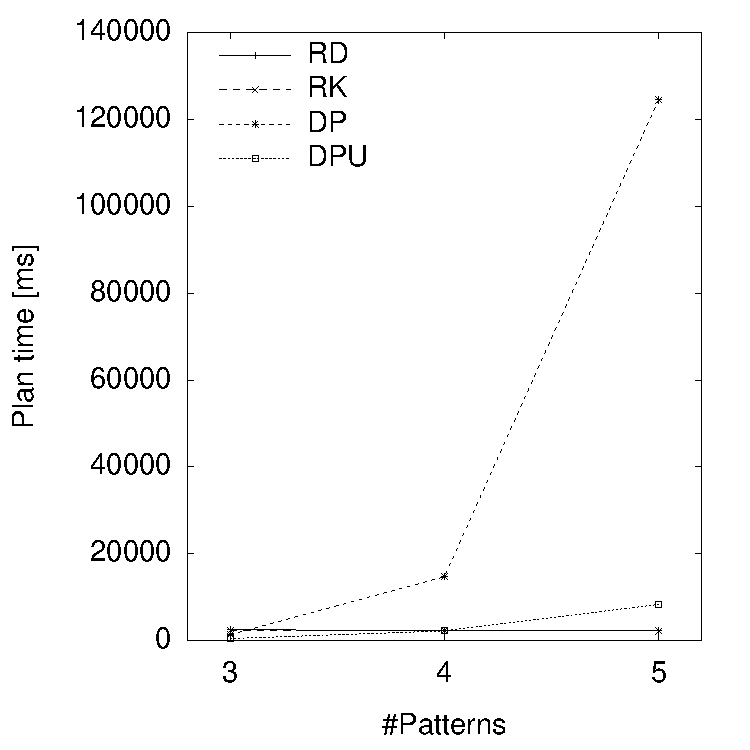
\includegraphics[width=0.49\linewidth]{figs/pareto_plan_tp.pdf}
%   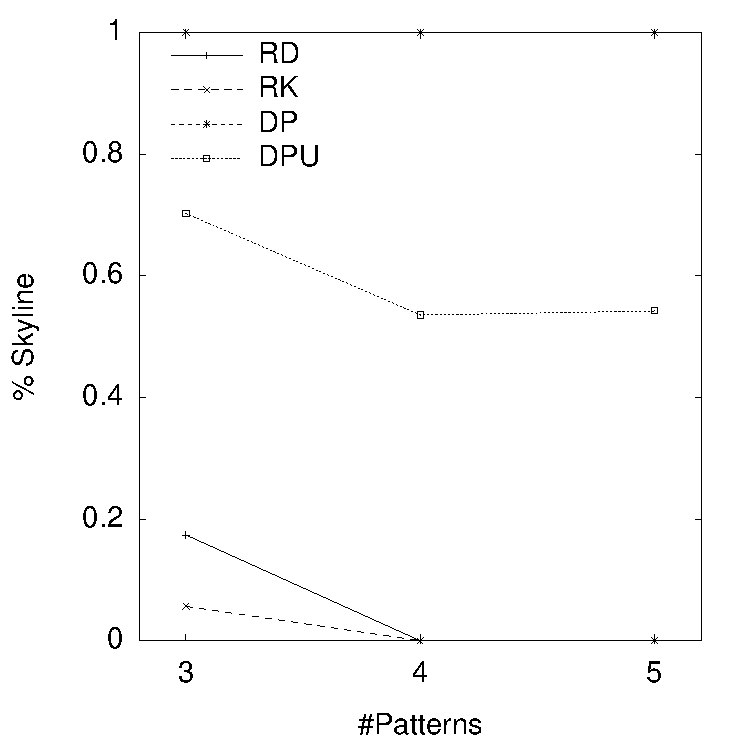
\includegraphics[width=0.49\linewidth]{figs/plans_skyline_by_tp.pdf}
%   \caption{Effect of query size on a) planning time and b) skyline
%     fractions ($b=0.8, m=2000$).}
%   \label{fig:pareto_tp}
% \end{figure}

\textbf{Effect of Sharing Benefit.} Figs.~\ref{fig:pareto_sharing}a+b
show the planning time and skyline fractions for different values of $b$. We see in Fig.~\ref{fig:pareto_sharing}a that planning times for systems without operator sharing (DPS, RD and RK) are not affected by $b$. 
%This is not surprising, given they because these planners do not take the
%sharing benefit into account.

For DP, planning time increases with higher sharing
benefits, namely from 36.7s for $b=0.1$ to 47.7s for $b=0.8$.  This is because cost bounds
are more loose with increasing benefit, and thus less plans can be pruned. 
DPU's planning time exhibits the opposite behavior, decreasing from 13.2s ($b=0.1$) to 3.8s
($b=0.8$). Compared to DP, DPU does not incur the cost of estimating bounds, and also, does not have the problem of loose bounds. Higher benefits only create steeper cost gradient
between plans, thus resulting in more plans that can be pruned.

Not taking precise bounds into account however has a negative effect on the optimality of plans. Fig.~\ref{fig:pareto_sharing}b illustrates that DPU produces a smaller fraction of skyline plans. This is because with higher sharing benefit, the deviation of bound estimates employed by DPU from the actual bounds becomes higher.  

%This is
%due to the fact that DPU does not take the effect of operating sharing
%into account, leading to worse results the more pronounced the
%influence of the sharing benefit is. The other approaches, DPS, RD and
%RK, are not affected by the sharing benefit as the benefit is not
%taken into account during planning.

\begin{figure}[htb]
  \vspace{-0.3cm}
  \centering
  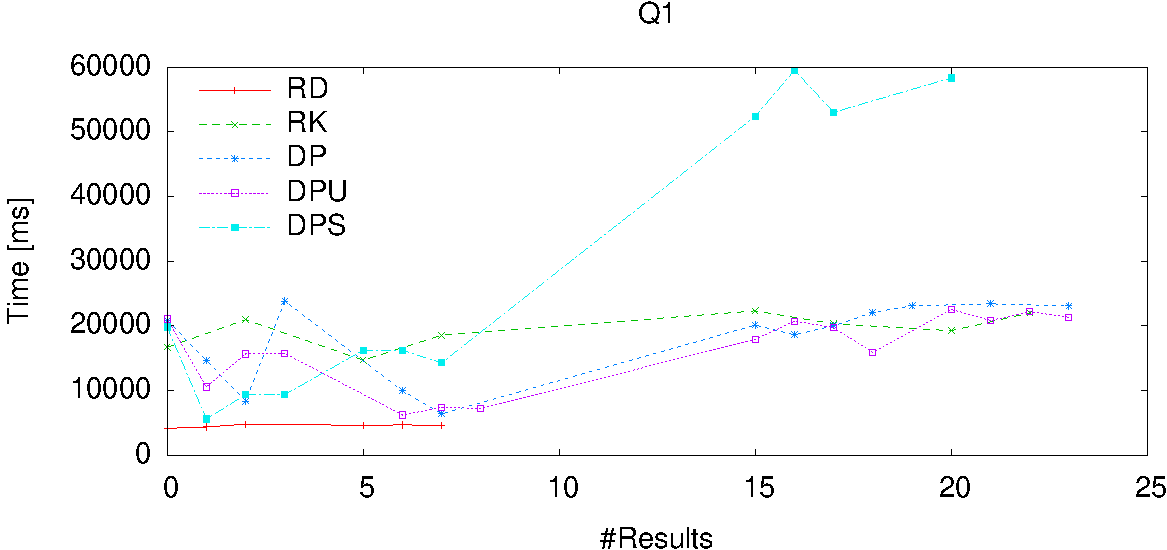
\includegraphics[width=0.82\linewidth]{figs/pareto_exec_0_q2-crop.pdf}
  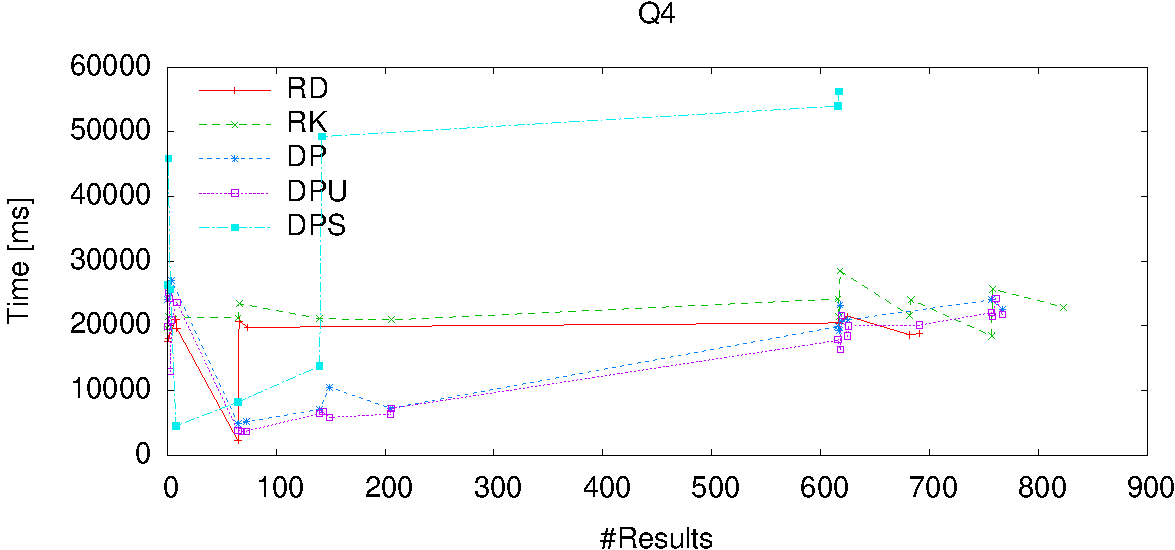
\includegraphics[width=0.82\linewidth]{figs/pareto_exec_0_q19-crop.pdf}
%  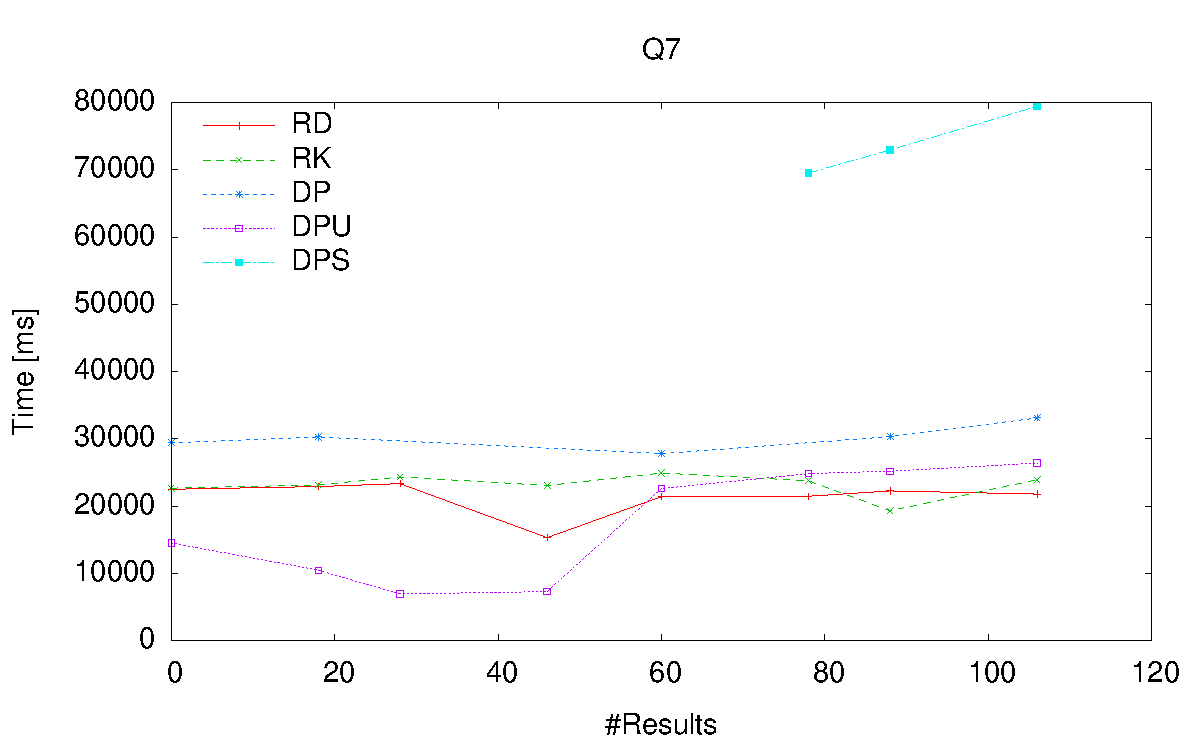
\includegraphics[width=0.32\linewidth]{figs/pareto_exec_0_q7.pdf}
  \caption{Execution times of query plans for queries Q1 and Q4.}
  \label{fig:exec}
  \vspace{-0.6cm}
\end{figure}


\textbf{Cost-Result Trade-off.} We analyze the cost-result trade-off
by studying the times needed for producing different number of
results. We selected two extreme queries. While Q1 produces only 24
results, Q4 yields 836 results. We randomly chose 20\% of the plans
generated by each system for these queries. We execute all of them and
record the total time (planning and processing). Fig.~\ref{fig:exec}
shows the results for both queries. Each point represents the
average total time of all plans that produce a particular number of
results. For example, all DP plans for query Q4 that produce 140
results have an average total query time of 7.1s. Since planning time
is the same for all query plans that are produced by the same system,
differences between total times of query plans for one system reflect
the different processing costs needed to produce different number of
results.

The systems DP, DPU and DPS, which optimize for both objectives, are
able to reduce total processing times, when fewer results have to be
produced. For both, Q1 and Q4, there is a trend that total times
increase with the number of results. For Q1, DP and DPU needed
$\sim$7s for computing 7 results, while they needed $\sim$21s to
compute $\sim$23 results. For Q4, they needed $\sim$4s and $\sim$21s
for computing $\sim$70 and $\sim$770 results, respectively.

No matter the amount of results, the other two systems, with a few
exceptions, needed $\sim$20s. One exception is Q1, where none of RD's
plans produces more than 7 results, resulting in much lower times
compared to the other systems.

This is reflected in the comparative results. DP and DPU provide
better performance than RD and RK when fewer results are needed.  For
example, to produce 7 results for Q1, DP and DPU require only 35\% of
the time RK needed to produce the same amount of result. Similarly,
for Q4, DP and DPU requires only 35\% of the total time of RK, when
205 results have to be produced.

Compared to DP and DPU, DPS query times increase substantially when a
larger amount of results is needed. This clearly indicates that the
use of operator sharing translates to better total performance.
%While DPU is able to outperform the baselines RK and RD for query Q7,
%the larger overhead of DP leads to a worse total average for all
%result sizes. The benefit of DPU is more pronounced for plans that
%produce fewer results, for 28 results DPU requires only 28\% of the
%time that plans for RK and RD need.

Even when computing only few results, we note that total processing
time may be high for DP, DPU, and DPS in a few cases. Most evident is
the case where these systems needed more than 20s even though the
results produced are empty. We observe this is due to the fact that
the employed cardinality estimation procedure does not take
dependencies between sources into account. Better treatment of this
and more sophisticated join size estimates
\cite{spiegel_graph-based_2006} can help to avoid empty and suboptimal
plans that result from incorrect cardinality and cost bounds.
%Here, a more sophisticated method for cardinality estimation
%would help avoid generating empty plans.











%Tab.~\ref{tab:exectimes} shows the average total query times for
%all systems for all three queries.

% sqlite> select system,avg(t_plan+t_execute) from runs where b=0.8 and query='q2' and delay=0 group by system;
% dp|15810.3125
% dps|24779.7794117647
% dpu|15532.1785714286
% rand|4450.47596153846
% rank|18929.3333333333

% sqlite> select system,avg(t_plan+t_execute) from runs where b=0.8 and query='q7' and delay=0 group by system;      
% dp|29751.0277777778
% dps|75013.9090909091
% dpu|16421.2794117647
% rand|21933.95
% rank|23302.0

% sqlite> select system,avg(t_plan+t_execute) from runs where b=0.8 and query='Q9' and delay=0 group by system;     
% dp|18151.0384615385
% dps|31050.8214285714
% dpu|16669.8846153846
% rand|18244.5434782609
% rank|21884.4935897436

% sqlite> select query,system,avg(t_plan+t_execute) from runs where b=0.8 and query in ('q2', 'q7', 'Q9') and delay=1500 group by query,system order by query;                                                                        
% Q9|dp|22841.4871794872
% Q9|dps|35001.9166666667
% Q9|dpu|20911.262195122
% Q9|rand|23130.6666666667
% q19|rank|26869.314516129
% q2|dp|20703.0909090909
% q2|dps|29921.3793103448
% q2|dpu|21166.1097560976
% q2|rand|23554.1111111111
% q2|rank|25453.0075757576
% q7|dp|36376.4537037037
% q7|dps|97149.75
% q7|dpu|30350.3928571429
% q7|rand|27545.1532258065
% q7|rank|27654.7661290323

%\begin{table}[htb]
%  \centering
%  \begin{tabular}{l|r|r|r|r|r}
%        & DP   & DPU  & DPS  & RD   & RK   \\
%    \hline
%    Q2  & 15.8 & 15.5 & 24.8 & 4.5  & 19.9 \\
%    Q7  & 29.8 & 16.4 & 75.0 & 21.9 & 23.3 \\
%    Q19 & 18.2 & 16.7 & 31.1 & 18.2 & 21.9 \\
%  \end{tabular}
%  \caption{Average total query times (in seconds) for all plans of queries Q2, Q7, Q19.}
%  \label{tab:exectimes}
%\end{table}



% First, we see that the RD baseline does not always find plans that
% produce all results (Q2, Q19), whereas RK is able to produce all
% results as RK prefers sources that contain many triples matching query
% triple patterns. DPS overall has the worst execution time, showing the
% large benefit of operator sharing. For queries Q2 and Q10 plans of DP
% and DPU generall perform better than the baselines, especially when
% only partial results are reported. For Q7, only DPU performs better
% whereas here the higher overhead leads to worse performance for DPU.

% Fig.~\ref{fig:exec_q7} shows the execution
% times and number of results for 20\% of plans (randomly chosen) for
% queries Q2, Q7 and Q19 for all approaches. 

% We see that plans that produce less results
% in general have shorter execution times. In order to find all 106
% query results, the fastest plan takes 17.9 seconds; producing a subset
% of 46 results requires only 4.3 seconds.

%%% Local Variables: 
%%% mode: latex
%%% TeX-master: "paper"
%%% End: 
